%\section{The differentiation operator}
\begin{python0}
from solutions import *; clear() 
\end{python0}

A useful operator on power series is \defone{differentiation}:
\begin{align*}
\frac{d}{dx} \ \sum^\infty_{n = 0} a_n x^n 
&= \sum_{n = 0}^\infty a_n \frac{d}{dx} x^n \\
&= \sum_{n=1}^\infty na_n x^{n-1} \\
&= \sum_{n = 0}^\infty (n+1)a_{n+1} x^n 
\end{align*}

Applying operator to the geometric series 
\[
\sum_{n=0}^\infty x^n = \frac{1}{1-x}
\]
we get
\[
\frac{d}{dx} \ \sum_{n=0}^\infty x^n = \frac{d}{dx} \ \frac{1}{1-x}
\]
i.e.
\[
\sum_{n=0}^\infty (n+1) x^n = \frac{1}{(1-x)^{2}}
\]

Of course we already know that from the formula:
\[
\sum_{n=0}^\infty \binom{k+n-1}{n} x^n = \frac{1}{(1-x)^{k}}
\]
Just substitute $k = 2$ and you get the above.
You can also think of the above computation as a proof of this
formula for the special case of $k = 2$.

Now let's step back and look at the differentiation operator.
This is what it does:
\begin{align*}
\frac{d}{dx} \ \sum^\infty_{n = 0} a_n x^n 
&= \sum_{n=1}^\infty na_n x^{n-1} \\
\end{align*}
Now instead of changing the index value like what we did above,
suppose I simply \lq\lq patch up'' the $n-1$ power of $x$ in the series
to $x^n$ by applying the shift-by-1 operator, i.e. multiplication by $x$:
\begin{align*}
x\frac{d}{dx} \ \sum^\infty_{n = 0} a_n x^n 
&= x\sum_{n=1}^\infty na_n x^{n-1} \\
&= \sum_{n=1}^\infty na_n x^{n}
\end{align*}
Of course this is the same as
\begin{align*}
x\frac{d}{dx} \ \sum^\infty_{n = 0} a_n x^n 
&= \sum_{n=0}^\infty na_n x^{n}
\end{align*}
since adding the term $n a_n x^n$ for $n=0$ is just adding $0$ to the series:
it adds nothing.

You see that operator
\[
x \frac{d}{dx}
\]
changes the power series as follows:
\begin{align*}
\sum^\infty_{n = 0} a_n x^n  \rightarrow
\sum_{n=0}^\infty (na_n) x^n
\end{align*}

I will refer to $\frac{d}{dx}$ and $x\frac{d}{dx}$ as differentiation
operators; it should be clear from the context which one I meant.
You can think of this special operator as multiplying the
coefficient with the corresponding power of $x$.

So what?

Well we know that
\[
\sum_{n=0}^\infty x^n = \frac{1}{1-x}
\]
Therefore
\[
\sum_{n=0}^\infty nx^n = x\frac{d}{dx} \, \frac{1}{1-x}
\]
Hence we've found a rational function for the generating function for
the sequence
\[
0, 1, 2, 3, 4, \ldots
\]
If we apply it again we get
\[
\sum_{n=0}^\infty n^2x^n = 
x\frac{d}{dx} 
\biggl( 
x\frac{d}{dx} \, \frac{1}{1-x}
\biggl)
\]
and we have the rational function for the squares:
\[
0^2, 1^2, 2^2, 3^2, 4^2, \ldots
\]

And what do these rational functions look like?
For the first case we have
\begin{align*}
\sum_{n=0}^\infty nx^n 
= x\frac{d}{dx} \, \frac{1}{1-x} \\
= \frac{x}{(1 - x)^2}
\end{align*}
And for the second case
\begin{align*}
\sum_{n=0}^\infty n^2x^n 
&= x\frac{d}{dx} \biggl( x \frac{d}{dx} \, \frac{1}{1-x} \biggr) \\
&= x\frac{d}{dx} \frac{x}{(1 - x)^2} \\
&= x \frac{(1-x)^2 - x(2(1-x)(-1))}{(1-x)^4} \\
&= x \frac{(1-x) + 2x}{(1-x)^3} \\
&= x \frac{1 + x}{(1-x)^3}
\end{align*}

In the next section we'll derive formulas for expressions such as
\[
0 + 1 + 2 + \cdots + n
\]
(you already know that this is $n(n+1)/2$) and
\[
0^2 + 1^2 + 2^2 + \cdots + n^2
\]
etc.


\newpage
\begin{ex}
The generating functions for cubes is
\[
\sum_{n=0}^\infty n^3 x^n
\]
Rewrite this as a rational function.
\end{ex}


\newpage
\begin{ex}
Rewrite the power series
\[
\sum_{n=0}^\infty n(n+1) x^n
\]
as a rational function in two different ways:
(1) use rational functions of power series that you already know
(2) use the differentiation operator.
\end{ex}


\newpage
\textsc{Differentiation.}

This is just a quick reminder of some formulas from Calc I.
For examples/exercises for review, 
you should refer to your calc textbook (or talk
to me - I'll give you some).

Actually we do not need a lot of differentiation rules.
Why? 
Because we're work mainly with 
rational functions.
Now rational functions are fractions of polynomials.
So of course you need to know how to take the derivative
of polynomials. If $n \neq 0$ and $c$ is a constant:
\[
\frac{d}{dx} x^n = n x^{n-1}, \,\,\,\,\ \frac{d}{dx} c = 0
\]
and 
\[
\frac{d}{dx} (f + g) = f' + g'
\]
Using the above rules you can differentiate any polynomial in $x$:
\begin{align*}
\frac{d}{dx} (2 + 3x + 5x^2 + 7x^3)
&= \frac{d}{dx} 2 + \frac{d}{dx} (3x) +  \frac{d}{dx}(5x^2) + 
\frac{d}{dx} (7x^3) \\
&= 0 + 3 +  10x + 21x^2
\end{align*}
and of course for a polynomial of degree $d$, we have
\[
\frac{d}{dx} \sum_{n=0}^d a_n x^n = \sum_{n=1}^d na_nx^{n-1}
\]
Since you have fractions, of course you need to know 
the quotient rule for differentiation:
\[
\frac{d}{dx} \frac{u}{v} = 
\frac{u' v - uv'}{v^2}
\]
where $u'$ is the same as $\frac{du}{dx}$.
For instance
\[
\frac{d}{dx} \ \frac{x^3}{(1 - x^2)(x+1)^2}
=
\frac{
\frac{d}{dx}(x^3) \cdot (1 - x^2)(x+1)^2
- x^3 \cdot \frac{d}{dx} \bigl( (1 - x^2)(x+1)^2 \bigr)
}
{\bigl( (1 - x^2)(x+1)^2 \bigr)^2}
\]
However note that quotients can also be computed using
the product rule since
\[
\frac{d}{dx} \ \frac{x^3}{(1 - x^2)(x+1)^2}
=
\frac{d}{dx} \ 
\biggl(
x^3 \cdot \bigl( (1 - x^2)(x+1)^2 \bigr)^{-1}
\biggr)
\]
In many cases the polynomials are powers of polynomial
(example: $(1 - x)^5$). 
Obviously you can expand the power to get a 
polynomial using binomial theorem.
But it's a lot faster to use the chain rule:
\[
\frac{d}{dx} f(g(x)) = f'(g(x)) g'(x)
\]
For instance
\[
\frac{d}{dx} \ (1-x)^5 = 5(1-x)^4 \cdot (-1)
\]
or
\[
\frac{d}{dx} \ (7x^2-3x^6)^5 = 5(1-x)^4 \cdot (14x - 18x^5)
\]
Note that using the chain rule guarantees that the resulting
polynomial in this case remains factored.

You should refer to your calc 1 textbooks for details and examples.

\newpage
\subsection*{Solutions}

\newpage
\section*{Solutions}
Solution to Exercise \ref{ex:dfa0}\labeltext{}{sol:dfa0}.

\tinysidebar{\debug{exercises/{dfa0/answer.tex}}}

    Solution not provided.
    

\newpage

Solution to Exercise \ref{ex:dfa1}\labeltext{}{sol:dfa1}.

\tinysidebar{\debug{exercises/{dfa1/answer.tex}}}
  The ID computation is
  \begin{align*}
    (q_0, aba)
    &\vdash (\delta(q_0, a), ba) = (q_0, ba) \\ 
    &\vdash (\delta(q_0, b), a) = (q_1, a) \\
    &\vdash (\delta(q_1, a), \ep) = (q_0, \ep)
  \end{align*}
  $q_0$ is not an accept state. Therefore $aba$ is not accepted.


\newpage

Solution to Exercise \ref{ex:dfa4}\labeltext{}{sol:dfa4}.

\tinysidebar{\debug{exercises/{dfa4/answer.tex}}}

    Solution not provided.
    

\newpage

Solution to Exercise \ref{ex:dfa5}\labeltext{}{sol:dfa5}.

\tinysidebar{\debug{exercises/{dfa5/answer.tex}}}

    Solution not provided.
    

\newpage

Solution to Exercise \ref{ex:implementing-a-single-dfa0}\labeltext{}{sol:implementing-a-single-dfa0}.

\tinysidebar{\debug{exercises/{implementing-a-single-dfa0/answer.tex}}}

    Solution not provided.
    

\newpage

Solution to Exercise \ref{ex:nfastatediag0}\labeltext{}{sol:nfastatediag0}.

\tinysidebar{\debug{exercises/{nfastatediag0/answer.tex}}}

    Solution not provided.
    

\newpage

Solution to Exercise \ref{ex:nfastatediag1}\labeltext{}{sol:nfastatediag1}.

\tinysidebar{\debug{exercises/{nfastatediag1/answer.tex}}}

    Solution not provided.
    

\newpage

Solution to Exercise \ref{ex:nfastatediag2}\labeltext{}{sol:nfastatediag2}.

\tinysidebar{\debug{exercises/{nfastatediag2/answer.tex}}}

    Solution not provided.
    

\newpage

Solution to Exercise \ref{ex:nfastatediag3}\labeltext{}{sol:nfastatediag3}.

\tinysidebar{\debug{exercises/{nfastatediag3/answer.tex}}}

    Solution not provided.
    

\newpage

Solution to Exercise \ref{ex:nfastatediag4}\labeltext{}{sol:nfastatediag4}.

\tinysidebar{\debug{exercises/{nfastatediag4/answer.tex}}}

    Solution not provided.
    

\newpage

Solution to Exercise \ref{ex:nfastatediag5}\labeltext{}{sol:nfastatediag5}.

\tinysidebar{\debug{exercises/{nfastatediag5/answer.tex}}}

    Solution not provided.
    

\newpage

Solution to Exercise \ref{ex:nfastatediag6}\labeltext{}{sol:nfastatediag6}.

\tinysidebar{\debug{exercises/{nfastatediag6/answer.tex}}}

    Solution not provided.
    

\newpage

Solution to Exercise \ref{ex:nfastatediag7}\labeltext{}{sol:nfastatediag7}.

\tinysidebar{\debug{exercises/{nfastatediag7/answer.tex}}}

    Solution not provided.
    

\newpage

Solution to Exercise \ref{ex:nfastatediag8}\labeltext{}{sol:nfastatediag8}.

\tinysidebar{\debug{exercises/{nfastatediag8/answer.tex}}}

    Solution not provided.
    

\newpage

Solution to Exercise \ref{ex:nfastatediag9}\labeltext{}{sol:nfastatediag9}.

\tinysidebar{\debug{exercises/{nfastatediag9/answer.tex}}}

    Solution not provided.
    

\newpage

Solution to Exercise \ref{ex:nfastatediag10}\labeltext{}{sol:nfastatediag10}.

\tinysidebar{\debug{exercises/{nfastatediag10/answer.tex}}}

    Solution not provided.
    

\newpage

Solution to Exercise \ref{ex:nfastatediag11}\labeltext{}{sol:nfastatediag11}.

\tinysidebar{\debug{exercises/{nfastatediag11/answer.tex}}}

    Solution not provided.
    

\newpage

Solution to Exercise \ref{ex:nfastatediag12}\labeltext{}{sol:nfastatediag12}.

\tinysidebar{\debug{exercises/{nfastatediag12/answer.tex}}}

    Solution not provided.
    

\newpage

Solution to Exercise \ref{ex:nfastatediag13}\labeltext{}{sol:nfastatediag13}.

\tinysidebar{\debug{exercises/{nfastatediag13/answer.tex}}}

    Solution not provided.
    

\newpage

Solution to Exercise \ref{ex:nfa0}\labeltext{}{sol:nfa0}.

\tinysidebar{\debug{exercises/{nfa0/answer.tex}}}
The formal definition of this NFA is $(\Sigma, Q, q_0, \delta, F)$ where
\begin{tightlist}
\li $\Sigma = \{a,b\}$
\li $Q = \{q_0\}$
\li $\delta$ is the function
\[
\delta : Q \times \Sigma_\epsilon \rightarrow P(Q)
\]
given by
\begin{align*}
  \delta(q_0, \epsilon) &= \{\} \\
  \delta(q_0, a) &= \{\} \\
  \delta(q_0, b) &= \{\} 
\end{align*}
\end{tightlist}


\newpage

Solution to Exercise \ref{ex:nfa1}\labeltext{}{sol:nfa1}.

\tinysidebar{\debug{exercises/{nfa1/answer.tex}}}

    Solution not provided.
    

\newpage

Solution to Exercise \ref{ex:nfa2}\labeltext{}{sol:nfa2}.

\tinysidebar{\debug{exercises/{nfa2/answer.tex}}}

    Solution not provided.
    

\newpage

Solution to Exercise \ref{ex:nfa3}\labeltext{}{sol:nfa3}.

\tinysidebar{\debug{exercises/{nfa3/answer.tex}}}

    Solution not provided.
    

\newpage

Solution to Exercise \ref{ex:nfa4}\labeltext{}{sol:nfa4}.

\tinysidebar{\debug{exercises/{nfa4/answer.tex}}}

    Solution not provided.
    

\newpage

Solution to Exercise \ref{ex:nfa5}\labeltext{}{sol:nfa5}.

\tinysidebar{\debug{exercises/{nfa5/answer.tex}}}

    Solution not provided.
    

\newpage

Solution to Exercise \ref{ex:dfa-as-powerful-as-nfa0}\labeltext{}{sol:dfa-as-powerful-as-nfa0}.

\tinysidebar{\debug{exercises/{dfa-as-powerful-as-nfa0/answer.tex}}}
Here's the solution.
Let $\delta$ denote the transition function of $N$.
Note that 
\begin{align*}
  \delta(q_0, \epsilon) = \{\} \\
  \delta(q_0, a) = \{\} \\
  \delta(q_0, b) = \{\} 
\end{align*}
First of all the states are labeled as all the subsets of $\{q_0\}$.


\begin{center}
\begin{tikzpicture}[>=triangle 60,shorten >=0.5pt,node distance=2cm,auto,initial text=, double distance=2pt]
\node[state] (A) at (  0,  0) {$\{q_0\}$};
\node[state] (B) at (  3,  0) {$\{\}$};

\path[->]

;
\end{tikzpicture}
\end{center}
    


The start state is the $\epsilon$-closure of $\{q_0\}$.
However in $N$, there are no $\epsilon$--transitions out of 
$q_0$.
So the $\epsilon$-closure of $\{q_0\}$ is in fact $\{q_0\}$, i.e.
$\overline{\{q_0\}} = \{q_0\}$
The $\DFA$ is now this:


\begin{longtable}{|r||r|r|r|r|r|}
\hline 
         & $w_1$ & $w_2$ & $w_3$ & $w_4$ & $\ldots$ \\ \hline \hline 
$M_1$    &       &       &       &       &          \\ \hline 
$M_2$    &       &       &       &       &          \\ \hline 
$M_3$    &       &       &       &       &          \\ \hline 
$M_4$    &       &       &       &       &          \\ \hline 
$\ldots$ &       &       &       &       &          \\ \hline 
\end{longtable}
        


Now I will compute the $a$--transition of the state $\{q_0\}$.
Let $\delta^\DFA$ denote the transition function of the $\DFA$
that we're building.
Then
\begin{align*}
\delta( \{q_0, a\} ) 
&= \overline{ \bigcup_{q \in \{q_0\}} \delta(q, a)} \\
&= \overline{ \delta(q_0, a) } \\
&= \overline{ \emptyset } \\
&= \emptyset
\end{align*}
The (incomplete) $\DFA$ now looks like this:


\begin{longtable}{|r||r|r|r|r|r|}
\hline 
         & $w_1$ & $w_2$ & $w_3$ & $w_4$ & $\ldots$ \\ \hline \hline 
$M_1$    & 0     & 0     & 1     & 0     & ...      \\ \hline 
$M_2$    & 1     & 0     & 1     & 1     & ...      \\ \hline 
$M_3$    & 0     & 1     & 1     & 1     & ...      \\ \hline 
$M_4$    & 1     & 0     & 1     & 1     & ...      \\ \hline 
$\ldots$ &       &       &       &       &          \\ \hline 
\end{longtable}
        


Using the same reasoning we have

\begin{center}
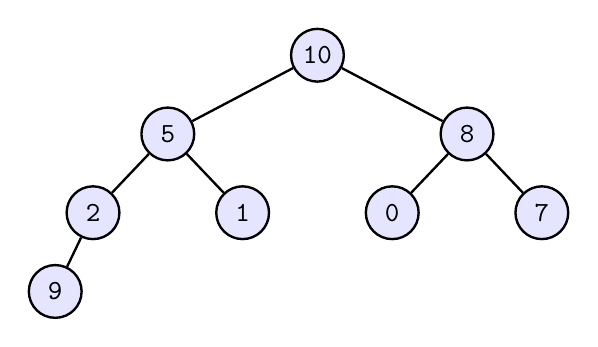
\begin{tikzpicture}

\fill[blue!10] (0.0, 0.0) circle (0.35);
\node [line width=0.03cm,black,minimum size=0.6699999999999999cm,draw,circle] at (0.0,0.0)(10){};\draw (0.0, 0.0) node[color=black] {\texttt{10}};
\fill[blue!10] (-1.9, -1.0) circle (0.35);
\node [line width=0.03cm,black,minimum size=0.6699999999999999cm,draw,circle] at (-1.9,-1.0)(5){};\draw (-1.9, -1.0) node[color=black] {\texttt{5}};
\fill[blue!10] (1.9, -1.0) circle (0.35);
\node [line width=0.03cm,black,minimum size=0.6699999999999999cm,draw,circle] at (1.9,-1.0)(8){};\draw (1.9, -1.0) node[color=black] {\texttt{8}};
\fill[blue!10] (-2.85, -2.0) circle (0.35);
\node [line width=0.03cm,black,minimum size=0.6699999999999999cm,draw,circle] at (-2.85,-2.0)(2){};\draw (-2.85, -2.0) node[color=black] {\texttt{2}};
\fill[blue!10] (-0.95, -2.0) circle (0.35);
\node [line width=0.03cm,black,minimum size=0.6699999999999999cm,draw,circle] at (-0.95,-2.0)(1){};\draw (-0.95, -2.0) node[color=black] {\texttt{1}};
\fill[blue!10] (0.95, -2.0) circle (0.35);
\node [line width=0.03cm,black,minimum size=0.6699999999999999cm,draw,circle] at (0.95,-2.0)(0){};\draw (0.95, -2.0) node[color=black] {\texttt{0}};
\fill[blue!10] (2.85, -2.0) circle (0.35);
\node [line width=0.03cm,black,minimum size=0.6699999999999999cm,draw,circle] at (2.85,-2.0)(7){};\draw (2.85, -2.0) node[color=black] {\texttt{7}};
\fill[blue!10] (-3.33, -3.0) circle (0.35);
\node [line width=0.03cm,black,minimum size=0.6699999999999999cm,draw,circle] at (-3.33,-3.0)(9){};\draw (-3.33, -3.0) node[color=black] {\texttt{9}};\draw[line width=0.03cm,black] (10) to  (5);
\draw[line width=0.03cm,black] (10) to  (8);
\draw[line width=0.03cm,black] (5) to  (2);
\draw[line width=0.03cm,black] (5) to  (1);
\draw[line width=0.03cm,black] (8) to  (0);
\draw[line width=0.03cm,black] (8) to  (7);
\draw[line width=0.03cm,black] (2) to  (9);
\end{tikzpicture}

\end{center}



It's easy to see that in the DFA, the $a$--
and $b$--transitions from the state $\{\}$ goes back to itself.
Therefore the completed DFA is this:


\begin{center}
\begin{tikzpicture}[>=triangle 60,shorten >=0.5pt,node distance=2cm,auto,initial text=, double distance=2pt]
\node[state,initial] (A) at (  0,  0) {$\{q_0\}$};
\node[state] (B) at (  3,  0) {$\{\}$};

\path[->]
(A) edge [bend left=0,pos=0.5,above] node {$a,b$} (B)
(B) edge [loop above] node {$a,b$} ()

;
\end{tikzpicture}
\end{center}
    



\newpage

Solution to Exercise \ref{ex:dfa-as-powerful-as-nfa1}\labeltext{}{sol:dfa-as-powerful-as-nfa1}.

\tinysidebar{\debug{exercises/{dfa-as-powerful-as-nfa1/answer.tex}}}

    Solution not provided.
    

\newpage

Solution to Exercise \ref{ex:dfa-as-powerful-as-nfa2}\labeltext{}{sol:dfa-as-powerful-as-nfa2}.

\tinysidebar{\debug{exercises/{dfa-as-powerful-as-nfa2/answer.tex}}}

    Solution not provided.
    

\newpage

Solution to Exercise \ref{ex:dfa-as-powerful-as-nfa3}\labeltext{}{sol:dfa-as-powerful-as-nfa3}.

\tinysidebar{\debug{exercises/{dfa-as-powerful-as-nfa3/answer.tex}}}

    Solution not provided.
    

\newpage

Solution to Exercise \ref{ex:dfa-as-powerful-as-nfa4}\labeltext{}{sol:dfa-as-powerful-as-nfa4}.

\tinysidebar{\debug{exercises/{dfa-as-powerful-as-nfa4/answer.tex}}}

    Solution not provided.
    

\newpage

Solution to Exercise \ref{ex:closure0}\labeltext{}{sol:closure0}.

\tinysidebar{\debug{exercises/{closure0/answer.tex}}}

    Solution not provided.
    

\newpage

Solution to Exercise \ref{ex:closure1}\labeltext{}{sol:closure1}.

\tinysidebar{\debug{exercises/{closure1/answer.tex}}}

    Solution not provided.
    

\newpage

Solution to Exercise \ref{ex:closure2}\labeltext{}{sol:closure2}.

\tinysidebar{\debug{exercises/{closure2/answer.tex}}}

    Solution not provided.
    

\newpage

Solution to Exercise \ref{ex:closure3}\labeltext{}{sol:closure3}.

\tinysidebar{\debug{exercises/{closure3/answer.tex}}}

    Solution not provided.
    

\newpage

Solution to Exercise \ref{ex:closure4}\labeltext{}{sol:closure4}.

\tinysidebar{\debug{exercises/{closure4/answer.tex}}}

    Solution not provided.
    

\newpage

Solution to Exercise \ref{ex:closure5}\labeltext{}{sol:closure5}.

\tinysidebar{\debug{exercises/{closure5/answer.tex}}}

    Solution not provided.
    

\newpage

Solution to Exercise \ref{ex:closure6}\labeltext{}{sol:closure6}.

\tinysidebar{\debug{exercises/{closure6/answer.tex}}}

    Solution not provided.
    

\newpage

Solution to Exercise \ref{ex:closure7}\labeltext{}{sol:closure7}.

\tinysidebar{\debug{exercises/{closure7/answer.tex}}}

    Solution not provided.
    

\newpage

Solution to Exercise \ref{ex:closure8}\labeltext{}{sol:closure8}.

\tinysidebar{\debug{exercises/{closure8/answer.tex}}}

    Solution not provided.
    

\newpage

Solution to Exercise \ref{ex:closure9}\labeltext{}{sol:closure9}.

\tinysidebar{\debug{exercises/{closure9/answer.tex}}}

    Solution not provided.
    

\newpage

Solution to Exercise \ref{ex:closure10}\labeltext{}{sol:closure10}.

\tinysidebar{\debug{exercises/{closure10/answer.tex}}}

    Solution not provided.
    

\newpage

Solution to Exercise \ref{ex:closure11}\labeltext{}{sol:closure11}.

\tinysidebar{\debug{exercises/{closure11/answer.tex}}}

    Solution not provided.
    

\newpage

Solution to Exercise \ref{ex:closure12}\labeltext{}{sol:closure12}.

\tinysidebar{\debug{exercises/{closure12/answer.tex}}}

    Solution not provided.
    
 % input solutions.tex
